% \documentclass[svgnames]{article}
% To make png: pdftopng -r 900 -alpha LucasBoston.pdf temp.png
\documentclass[svgnames,convert={density=900,size=720x600,outext=.png}]{standalone}
\usepackage{tikz}
\usetikzlibrary{calc,trees,positioning,arrows,chains,shapes.geometric,backgrounds,
  decorations.pathreplacing,decorations.pathmorphing,shapes,snakes,automata,
  matrix,shapes.symbols,mindmap,shadows,petri}
% \renewcommand{\rmdefault}{phv} % Arial
% \renewcommand{\sfdefault}{phv} % Arial
% \usepackage{amsmath} % to allow Sans font in math


\begin{document}
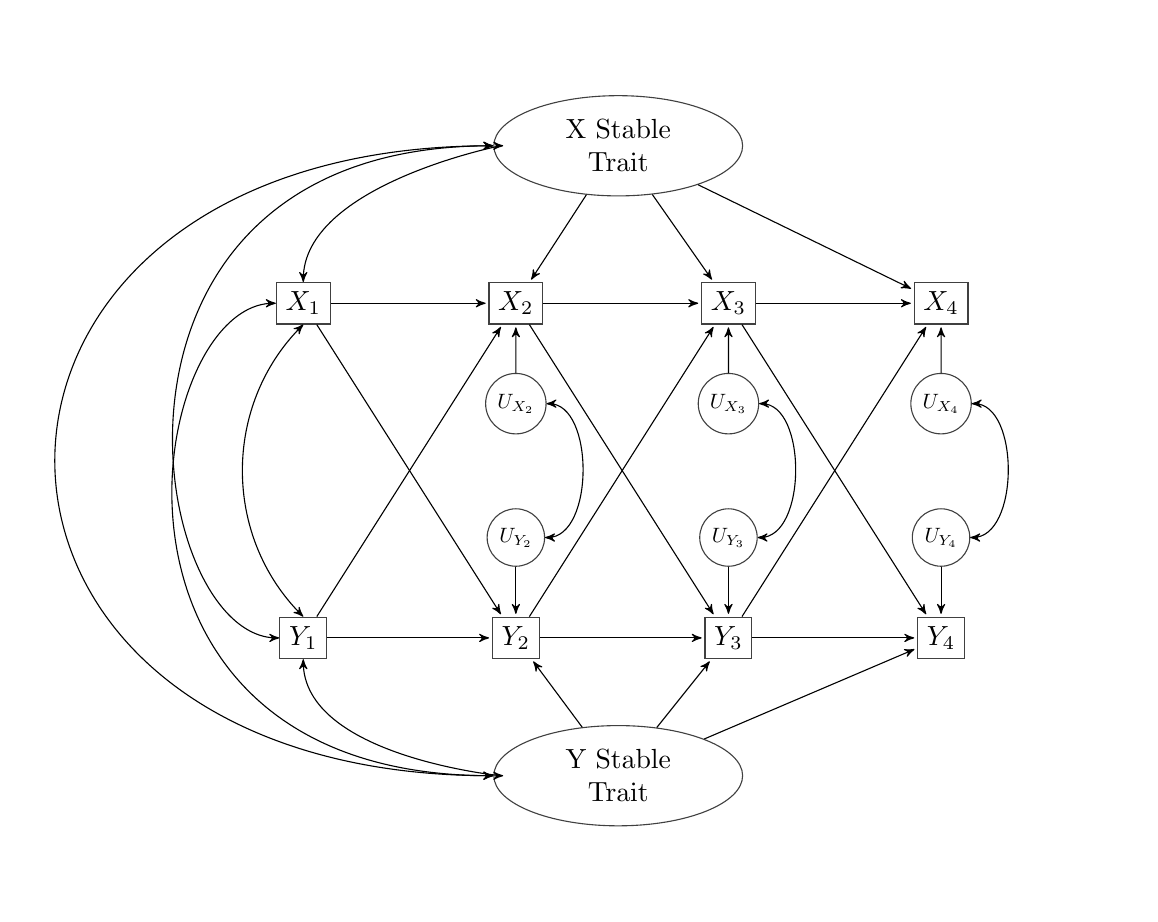
\begin{tikzpicture}[node distance=1.8cm,>=stealth',bend angle=45,auto]
  \useasboundingbox (-8,-9) rectangle (6,2);
  \tikzset{
    latentTrait/.style={ellipse,draw=black!75,minimum size=5mm, text width=20mm, align=center},
    latentAR/.style={ellipse,draw=black!75,minimum size=7mm},
    observed/.style={rectangle,draw=black!75,minimum size=5mm, align=center},
    error/.style={circle,draw=black!75,minimum size=.9mm},
    errorAR/.style={circle,draw=black!75,minimum size=1mm, node distance=.73cm},
    state/.style={circle,draw=black!75,minimum size=1mm, scale=.75, align=center, node distance=1.7cm},
    hspace/.style={node distance=2.7cm},
    vspace/.style={node distance=4.25cm},
    % edge styles
    indicatorDist/.style={node distance=1.2cm},
    errorDist/.style={node distance=.73cm},
    newARDist/.style={node distance=1.2cm},
    stabDist/.style={node distance=1cm},
    % label styles
    constraints/.style={scale=.75,above},
    constraintsb/.style={scale=.75,below},
    constraintsl/.style={scale=.75,left},
    constraintsr/.style={scale=.75,right}
  }


  % Labels
  %%% STARTS
  
  % X Vars (Health)

  \node [latentTrait] (health) at (-.5,.5)                        {X Stable Trait};
  \node [observed] (t1) at (-4.5,-1.5)                        {$X_1$};


  

  
  \node [observed,hspace] (t2) [right of=t1]                         {$X_2$}
  edge [pre] node[constraints] {} (health)
  edge [pre] node[constraintsl] {} (t1);

  \node [state] (s2) [below of=t2] {$U_{X_2}$}
  edge [post] node[constraintsl] {} (t2);

  
  \node [observed, hspace] (t3) [right of=t2]                         {$X_3$}
  edge [pre] node[constraints] {} (health)
  edge [pre] node[constraintsl] {} (t2);

  \node [state] (s3) [below of=t3] {$U_{X_3}$}
  edge [post] node[constraintsl] {} (t3);

  
  \node [observed, hspace] (t4) [right of=t3]                         {$X_4$}
  edge [pre] node[constraints] {} (health)
  edge [pre] node[constraintsl] {} (t3);

  \node [state] (s4) [below of=t4] {$U_{X_4}$}
  edge [post] node[constraintsl] {} (t4);


  
  % SWB
  \node [latentTrait] (SWB) [below of=health, node distance = 8cm]         {Y Stable Trait};
  \node [observed, vspace] (t1s) [below of=t1] {$Y_1$}
  %edge [<->] node[constraintsb] {} (SWB)
  edge [post] node[constraints] {} (t2);
  
  
  \node [observed, vspace] (t2s) [below of=t2]                        {$Y_2$}
  edge [pre] node[constraintsb] {} (SWB)
  edge [pre] node[constraintsl] {} (t1s)
  edge [pre] node[constraints] {} (t1)
  edge [post] node[constraints] {} (t3);
  
  \node [state] (sy2) [above of=t2s] {$U_{Y_2}$}
  edge [post] node[constraintsl] {} (t2s);

  
  \node [observed, vspace] (t3s) [below of=t3]                        {$Y_3$}
  edge [pre] node[constraintsb] {} (SWB)
  edge [pre] node[constraintsl] {} (t2s)
  edge [pre] node[constraints] {} (t2)
  edge [post] node[constraints] {} (t4);
  
  \node [state] (sy3) [above of=t3s] {$U_{Y_3}$}
  edge [post] node[constraintsl] {} (t3s);

  
  \node [observed,vspace] (t4s) [below of=t4]                        {$Y_4$}
  edge [pre] node[constraintsb] {} (SWB)
  edge [pre] node[constraintsl] {} (t3s)
  edge [pre] node[constraints] {} (t3);
  
  \node [state] (sy4) [above of=t4s] {$U_{Y_4}$}
  edge [post] node[constraintsl] {} (t4s);




  % Correlations
  \draw [<->] (SWB) .. controls +(left:9cm) and +
  (left:9cm) .. node[sloped,above] {} (health);

  \draw [<->] (SWB) .. controls +(left:7cm) and +
  (left:2cm) .. node[sloped,above] {} (t1);
  \draw [<->] (health) .. controls +(left:7cm) and +
  (left:2cm) .. node[sloped,above] {} (t1s);
  \draw [>->] (SWB) .. controls +(west:1.5cm) and +
  (south:1.5cm) .. node[] {} (t1s);
  \draw [>->] (health) .. controls +(west:1.5cm) and +
  (north:1.5cm) .. node[] {} (t1);

  \draw [<->] (t1.south) to [out=225,in=135] (t1s.north);
  

  
  \draw [<->] (sy2) .. controls + (right:1cm) and +
  (right:1cm) ..  (s2);
  \draw [<->] (sy3) .. controls + (right:1cm) and +
  (right:1cm) ..  (s3);
  \draw [<->] (sy4) .. controls + (right:1cm) and +
  (right:1cm) .. node[above,rotate=-90,scale=.75] {}  (s4);

  
\end{tikzpicture}
\end{document}